\mysubsection{Sarah Häfele}{Aufbau}

Die Installation besteht aus mehreren Hardware- und Software-Komponenten und soll hier mit Hilfe einer kurzen, modellhaften Übersicht, die den endgültigen Aufbau des Prototypen zeigt, skizziert werden. Die darauffolgenden Kapitel gehen anschließend näher auf die einzelnen Komponenten ein. Der Prototyp der Installation wurde am 20.01.2015 im Rahmen des \textit{Tag der Medien} der Fakultät Digitale Medien aufgebaut und getestet. Auf zwei Ebenen wurden Gerätschaften installiert, damit die Besucher schon beim Eintreten mit akustischen und visuellen Reizen konfrontiert und zum Mitmachen bewegt wurden. Abb.~\ref{fig:Aufbau}~(a) und \ref{fig:Aufbau} (b) zeigen Erdgeschoss und ersten Stock des Gebäudes.

\begin{figure}[htbp]
\subfigure[I-Bau, 1. Stock, Lichthof]{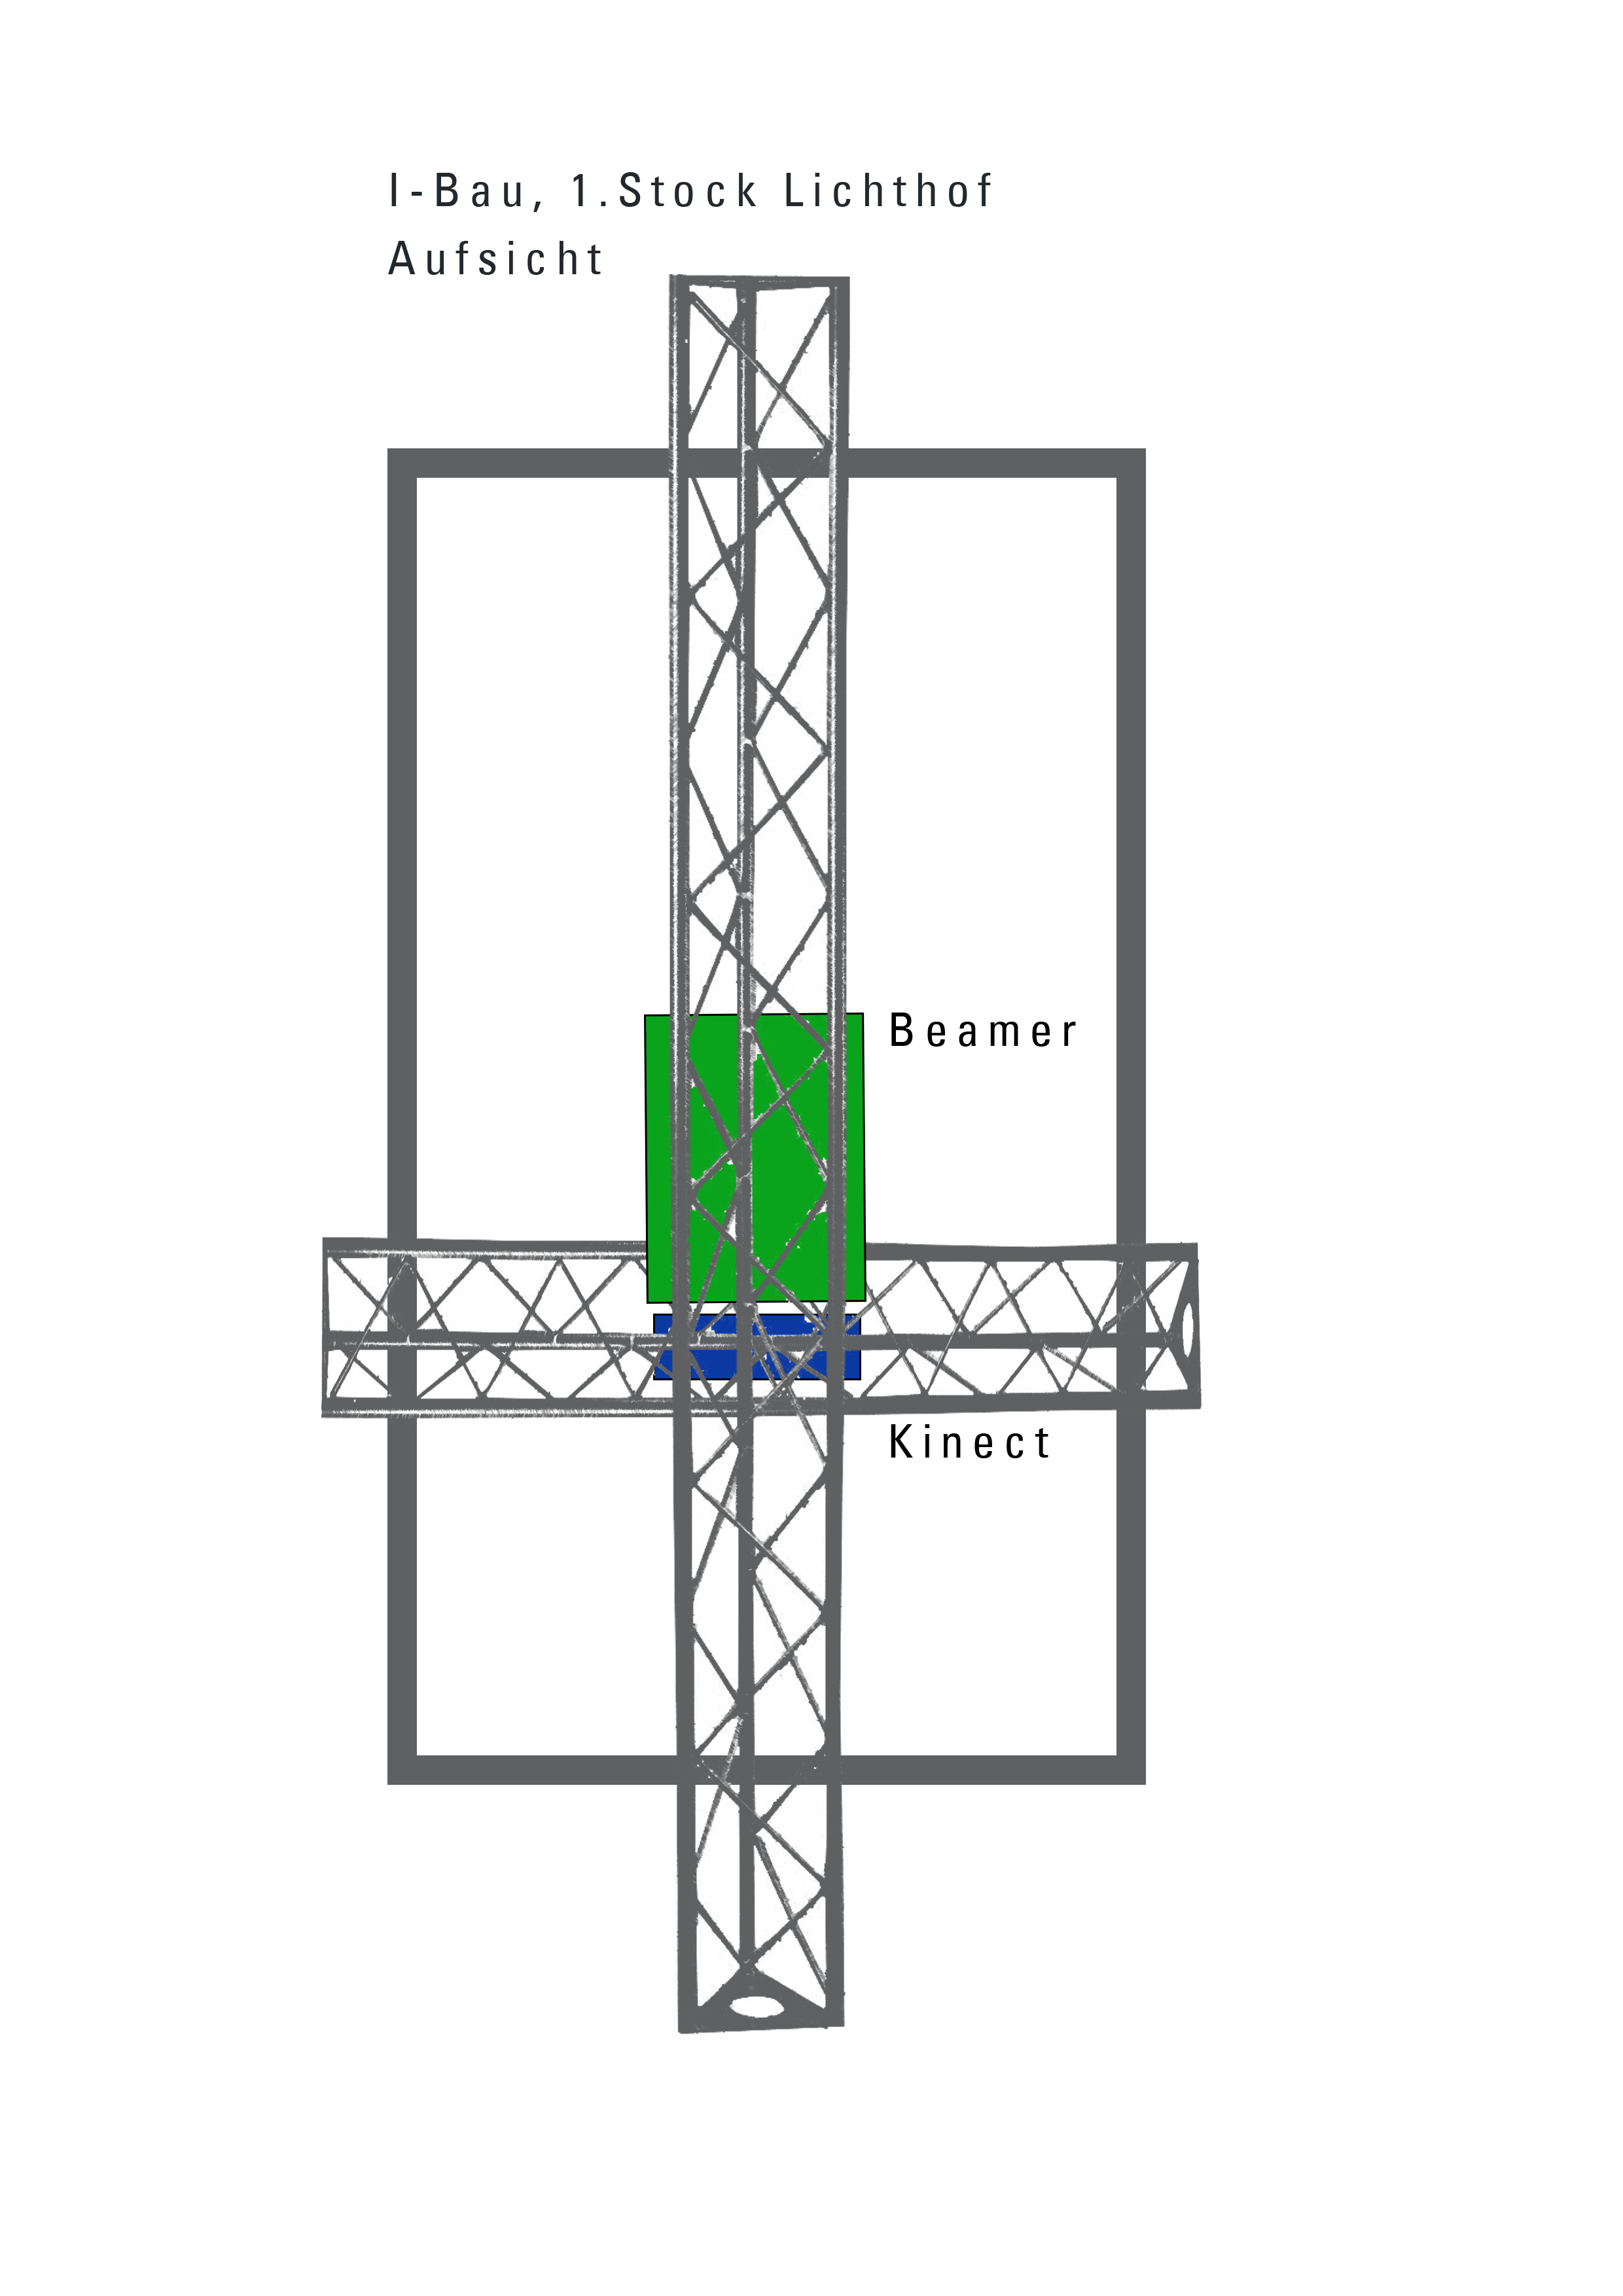
\includegraphics[width=0.49\textwidth]{images/ModelFirstFloor.png}}\hfill
\subfigure[I-Bau, Erdgeschoss]{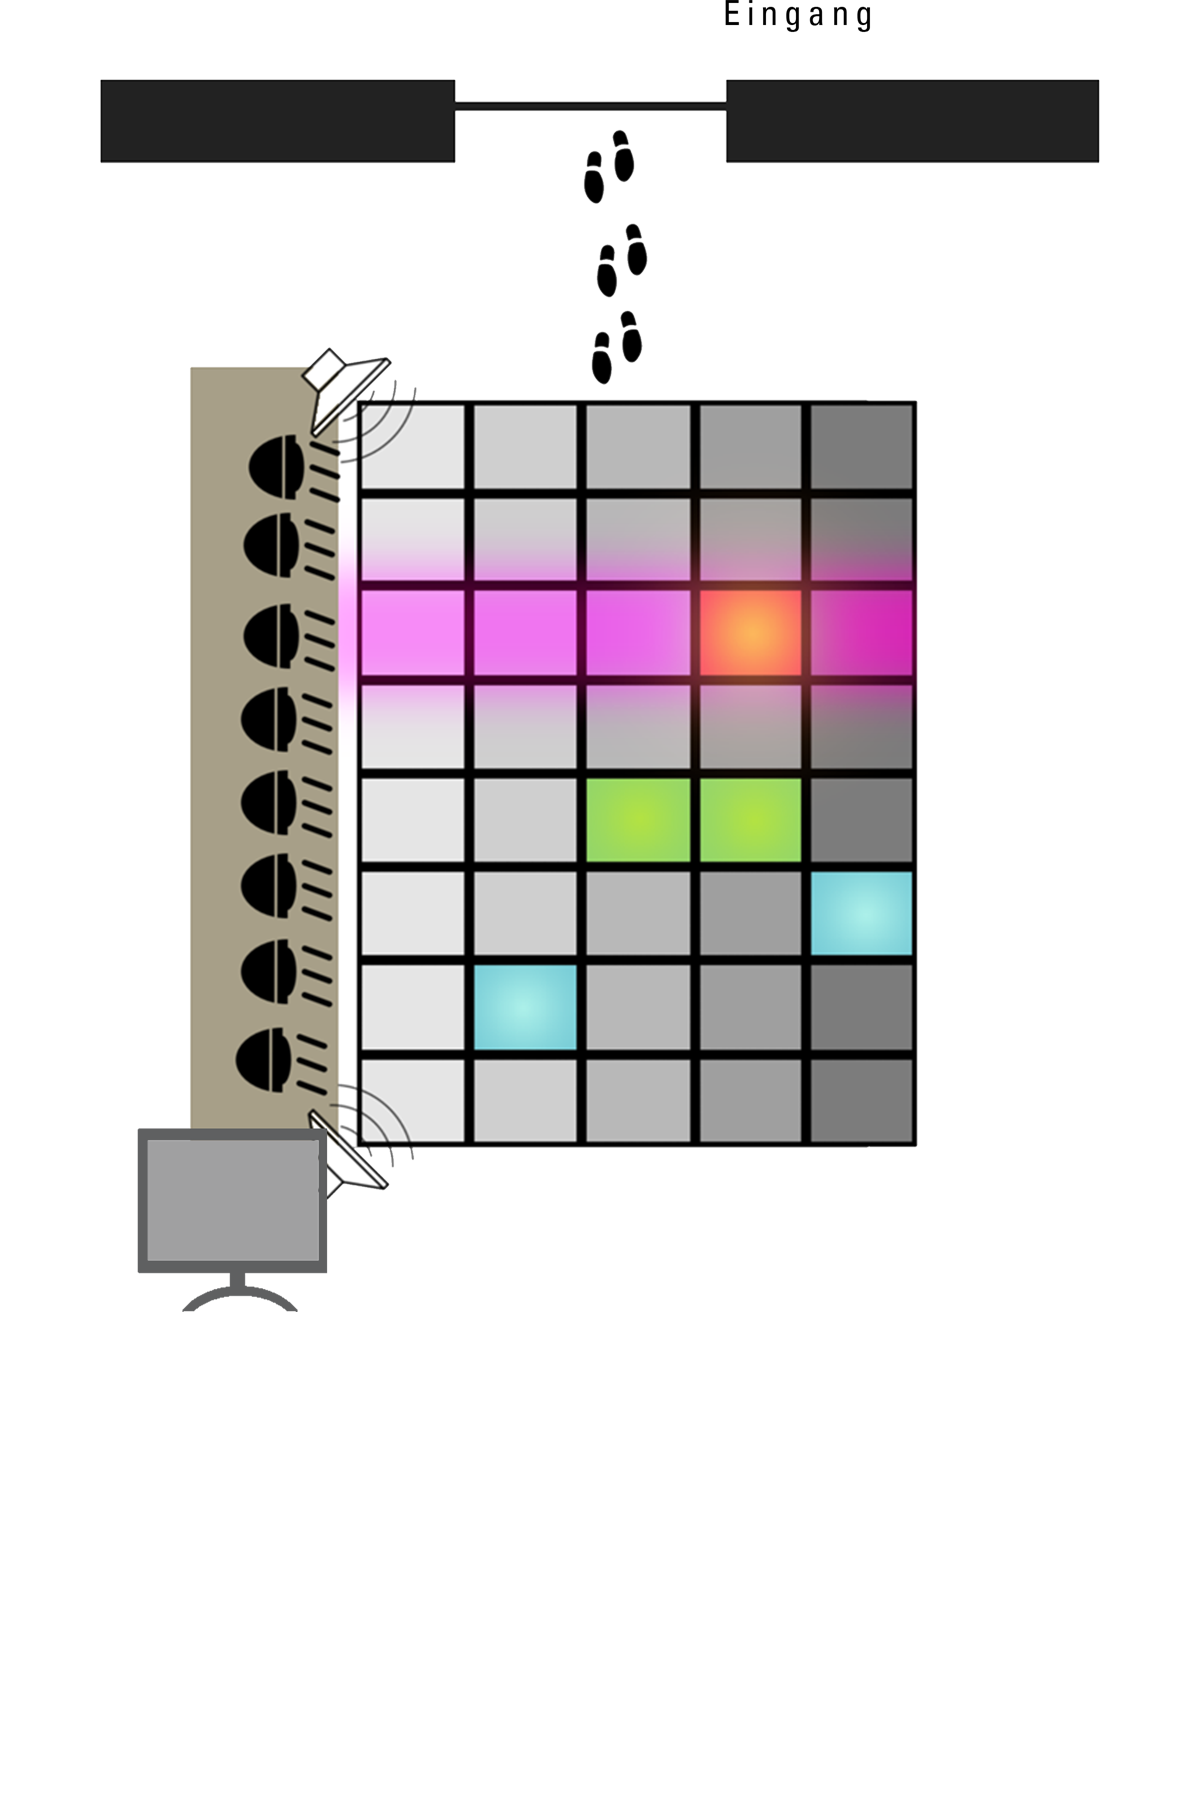
\includegraphics[width=0.49\textwidth]{images/ModelGroundFloor.png}}
\caption{Aufbau der Installation im I-Bau (Aufsicht)}
\label{fig:Aufbau}
\end{figure}

Im ersten Stockwerk hängt über dem Lichthof eine von zwei Stativen (sogenannte Traversenlifte) getragene sieben Meter lange Traverse, in deren Mitte ein \emph{Epson EB-4950WU}-Beamer (in der Abb. \ref{fig:Aufbau} (a) grün markiert), der durch eine speziell von der Werkstatt der Hochschule angefertigten Metallhalterung gehalten wird, in das Erdgeschoss des Gebäudes strahlt. Der Beamer, eine Leihgabe des Kreismedienzentrums Schwarzwald-Baar, kann mit seiner Helligkeit von bis zu 4.500 ANSI Lumen und eine Auflösung von 1920 x 1200 Pixeln den dunklen Boden des I-Baus mühelos ausleuchten und ist zudem für längere Betriebszeiten ausgerichtet. Durch die erhöhte Stellung der Traversenlifte hängt der Beamer sechs Meter über dem Erdgeschossboden. Angeschlossen ist der Beamer mittels HDMI an einen Computer, auf dem die Steuerung läuft.

Auf der Brüstung des Lichthofes liegt im 90° Winkel dazu eine zwei Meter lange Traverse, die durch von der Schreinerei der Hochschule angefertigte Holzhalterungen und durch sogenannte \emph{Doughty Clamps} fixiert wird. Sie wird nicht ganz mittig zu der längeren Traverse ausgerichtet, damit die mit Spannfix daran befestigte Microsoft Kinect (in der Abb. \ref{fig:Aufbau} (a) blau markiert) nicht das Bild des Beamers stört. Durch die direkte Anbringung auf dem Geländer des Lichthofes, hängt die Kinect auf 4,5 Meter Höhe und kann so optimal die Bewegungen der im Erdgeschoss befindlichen Personen aufnehmen. Zudem sind zwei Scheinwerfer (so genannte \textit{Revos}, in Abb. \ref{fig:Aufbau} (a) braun markiert) an der längeren Traverse links und rechts vom Beamer angebracht und versehen den Boden mit Lichteffekten, die automatisiert durch Sound gesteuert werden.

Im Erdgeschoss (siehe Abb. \ref{fig:Aufbau} (b)) wird durch den Beamer ein 5 x 8 flächiges Raster projiziert, welches die einzelnen Töne repräsentiert. Acht LED-Scheinwerfer untermalen die Rhythmuslinie, welche bestimmt, wann ein Ton abgespielt wird. Die Scheinwerfer sind durch ein DMX-Interface untereinander und mit dem Computer verbunden und werden durch ein eigenes Programm gesteuert (vgl. Abschnitt \ref{ssec:DMX}). Ein großer LED-Monitor zeigt den Besuchern Informationen an und dient zusätzlich als Motivation (vgl. auch Abschnitt \ref{ssec:CtA}). Die Musik wird durch einen mobilen, jedoch leistungsstarken Radiorekorder (\textit{Boombox} genannt) abgespielt. Diese ist ebenfalls über ein XLR-Kabel und mittels Adapter an den Computer angeschlossen.